\documentclass{article}

\usepackage{color}
\usepackage[draft]{todonotes}

\newcommand\mustafa[1]{\todo[color=green]{\textbf{Mustafa:} #1}}

\begin{document}
    \title{UPoA: A Scalable Untrusted Privacy-Preserving Transparency Overlay with Applications to Auditable Software Distribution}

    \maketitle
    \begin{abstract}
        Transparency overlays such as Certificate Transparency (CT) and Bitcoin seek to bring auditability to security-critical applications that rely on sets of authoritative messages. However such overlays tend to either have poor scalability (Bitcoin) or require trust in a set of distributed actors (CT), and trust-reducing CT protocols such as gossiping suffer from privacy and complexity issues.

        In this work, we present a general-purpose transparency overlay that builds on the untrusted nature of blockchains---or distributed ledgers---such as Bitcoin. By using blockchain transactions with relaxed validation constraints, we achieve high scalability for an untrusted privacy-preserving transparency overlay that detects but not prevents misbehaviour. Our overlay makes use of a blockchain for log commitments and Untrusted Proof of Auditability (UPoA), with monitors for detecting misbehaviour. We implement this for the application of auditable software distribution and we test it at scale on the Debian software repositories.
    \end{abstract}

    \section{Introduction}
    Critical Internet services are often provided by trusted third parties that have the ability to misbehave without being immediately detected---such as TLS certificate authorities that have issued unauthorised certificates for major websites.\cite{dangoodin2015}\cite{johnleyden2011}

    Consequently, a number of projects have emerged to bring transparency to Internet services. One of these projects is Certificate Transparency (CT), a framework for monitoring and auditing TLS certificates to make it possible to detect unauthorised certificates issued by certificate authorities.\cite{benlaurie2013}

    CT however still requires trust in a third party actor. The log servers that auditors communicate with to check that certificates have been logged are trusted, because they may misbehave by presenting a ``split view'' of their operations (i.e. log servers may say that they have seen a certificate to one auditor but not to other auditors).\cite{linusnordberg2015}

    CT "gossiping" protocols have therefore been drafted to help detect misbehaviour of log servers.\cite{linusnordberg2015}\cite{laurentchuat2015} This reduces but not eliminates the trust required in log servers, partly because gossip is not guaranteed to reach the wider Internet if a long-term man-in-the-middle attack takes place. This makes gossiping unsuitable for threat models where a device is connected to the same network for a long period of time and an adversary sits on the device's network (e.g. ISP). Additionally, CT gossiping suffers from a number of privacy problems and fingerprinting attacks.\cite{linusnordberg2015}\mustafa{Add note explaining why this is particularly unsuitable for transparent software distribution and introduce the problem space.}

    Bitcoin is decentralised peer-to-peer electronic cash system that takes a different approach to transparency. Instead of merely employing transparency to detect misbehaviour or placing trust in any actors, Bitcoin makes misbehaviour economically expensive by using an auditable untrusted consensus protocol based on proof-of-work---the blockchain. This prevents users from double spending their coins without access to 51\% of the processing power that generates proof-of-work in the network.\cite{satoshinakamoto2008}

    All full nodes (nodes that have the ability to bootstrap other nodes) in the peer-to-peer network that maintains the blockchain must store a copy of all the transactional data in the blockchain. This means adding new data to the blockchain is an expensive operation, making scalability while keeping the network decentralised a difficult problem. \mustafa{Add a citation about fees associated with storage size of transactions in systems like Ethereum.}

    Systems such as Certificate Transparency and the blockchain can be generalised as transparency overlays because they can adapted to provide transparency for any number of different applications.\cite{melissachase2016} For example, it is possible to define an electronic cash system based on a CT-like overlay where users trust a set of distributed actors\cite{melissachase2016} and centrally banked cryptocurrencies have been proposed using similar distributed schemes.\cite{georgedanezis2016}

    The tradeoff between different the approaches has been that a decentralised overlay is poorly scalable and expensive, but a distributed overlay is trusted.

    \subsection{Our Contributions}
    We contribute a unique, third type of transparency overlay where misbehaviour is detected (but not prevented) in an untrusted manner, by drawing on concepts from both types of decentralised and distributed approaches.\mustafa{Incomplete.}

    \subsection{Related Work}
    \section{Background}
    \section{Protocol}
    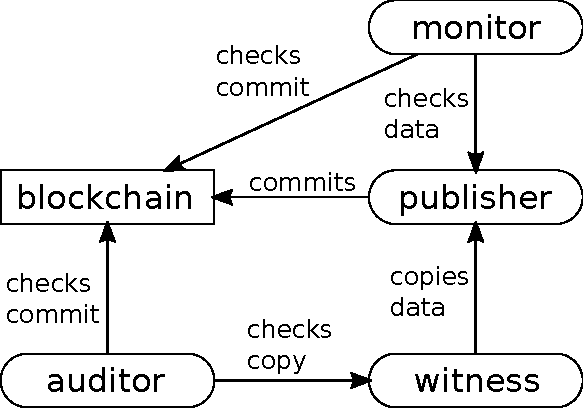
\includegraphics{architecture.pdf}

    \bibliography{upoa}
    \bibliographystyle{ieeetr}
\end{document}
